% https://tex.stackexchange.com/questions/428644/
\documentclass[border=5mm]{standalone}
\usepackage{tikz}
\usetikzlibrary{calc}
\usetikzlibrary{arrows.meta}
\begin{document}
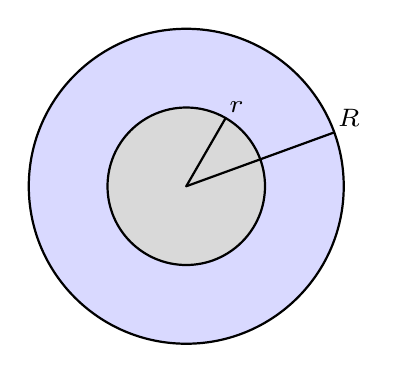
\begin{tikzpicture}[
  line cap=round,
  line join=round,
  >=Triangle,
  myaxis/.style={->,thick},
  every node/.style={scale=1.3}
]

% inner/outer circle: \fill before \draw
\fill [gray!30] (0,0) circle[radius=1];
\fill [blue!15, even odd rule] (0,0) circle[radius=1] circle[radius=2];
\draw [thick] (0,0) circle[radius=1];
\draw [thick] (0,0) circle[radius=2];

\begin{scope}[
  every node/.append style={
    circle,
    font=\scriptsize,
    inner sep=1pt
}]
  \draw [thick] (0,0) -- (60:1cm) node[anchor=225] {$r$};
  \draw [thick] (0,0) -- (20:2cm) node[anchor=225] {$R$};
\end{scope}

\end{tikzpicture}
\end{document}